\documentclass[UTF8, a4paper, 11pt]{article}
\usepackage{amssymb}
\usepackage{fontspec}
\usepackage{float}
\usepackage{amsmath}
\newtheorem{myDef}{Definition}
\usepackage{graphicx}
\usepackage{geometry}
\usepackage{listings}
\usepackage{xcolor}
\usepackage{caption,subcaption}
\geometry{scale=0.8}
\linespread{1.5}
\usepackage{hyperref}
\usepackage{color}
\usepackage{fontspec}
\usepackage{enumitem}
\usepackage[linesnumbered,boxed]{algorithm2e}    
\usepackage{xeCJK}
\usepackage{indentfirst} 
\graphicspath{{Pic/}} 	% 在于.tex同级的目录下创建名为pic的文件夹,存放图片


\setlength{\parindent}{2em}

\lstset{
    language={C},
    frame=shadowbox,
    breaklines=true,
    numbers=left,
    backgroundcolor=\color[RGB]{245,245,244},
    rulesepcolor=\color{red!20!green!20!blue!20},
    numberstyle={\color[RGB]{0,192,192}\tiny},
    basicstyle=\footnotesize \fontspec{Source Code Pro}
}
\setenumerate[1]{itemsep=0pt,partopsep=0pt,parsep=\parskip,topsep=0pt}
\setitemize[1]{itemsep=0pt,partopsep=0pt,parsep=\parskip,topsep=0pt}
\setdescription{itemsep=0pt,partopsep=0pt,parsep=\parskip,topsep=0pt}


\title{	
\normalfont \normalsize
\textsc{School of Data and Computer Science, Sun Yat-sen University} \\ [25pt] %textsc small capital letters
\rule{\textwidth}{0.5pt} \\[0.4cm] % Thin top horizontal rule
\huge Summary of Generative Adversarial Self-Imitation Learning\\ % The assignment title
\rule{\textwidth}{2pt} \\[0.5cm] % Thick bottom horizontal rule
\author{18308045 Zhengyang Gu}
\date{\normalsize\today}
}

\begin{document}
\maketitle
\tableofcontents
\newpage

\section{Theories}
\subsection{Policy Gradient}
\subsubsection{On-policy}
The purpose of policy gradient is to maximize the expected reward as follows:
$$\overline R_\theta=\sum_\tau R(\tau)p_\theta(\tau)=E_{\tau\sim p_\theta}[R(\tau)]$$
where $R(\tau)$ is the final reward of trajectory $\tau$ and $p_\theta$ is the probability of trajectory $\tau$.Therefore, we need to calculate its gradient to do
gradient ascent. The gradient of it can be calculated by:
$$\begin{aligned}
\nabla\overline R_\theta=&\sum_\tau R(\tau)\nabla p_\theta(\tau)\\
=&\sum_\tau R(\tau)p_\theta(\tau)\frac{\nabla p_\theta(\tau)}{p_\theta(\tau)}\\
=&\sum_\tau R(\tau)p_\theta(\tau)\nabla\log(p_\theta(\tau))\\
=&\mathbb{E}_{\tau\sim p_\theta} R(\tau)\nabla\log(p_\theta(\tau))
\end{aligned}$$
We can estimate the expectation using sampling, so we have:
$$\begin{aligned}
\nabla\overline R_\theta\approx&\frac1 N\sum_{n=1}^N R(\tau^n)\nabla\log(p_\theta(\tau^n))\\
=&\frac1 N\sum_{n=1}^N\sum_{t=1}^{T_n}R(\tau^n)\nabla\log(p_\theta(a_t^n|s_t^n))
\end{aligned}$$
where $N$ is the total number of samples, and $\tau^n$ is the $n$th sampled trajectory. Since the $R(\tau^n)$ is always positive, a biased sampling may cause
unexpected ascent of some bad trajectories whose rewards are lower than average reward. Therefore, we can add a baseline to it to penalize those bad trajectories,
as follows:
$$\nabla\overline R_\theta\approx\frac1 N\sum_{n=1}^N\sum_{t=1}^{T_n}(R(\tau^n)-b)\nabla\log(p_\theta(a_t^n|s_t^n))$$
where $b$ can be easily assigned $\frac1 N\sum_{n=1}^N R(\tau^n)$. Additionally, we can separately evaluate each action given a state in a trajectory, so we have:
$$\begin{aligned}
\nabla\overline R_\theta\approx&\frac1 N\sum_{n=1}^N\sum_{t=1}^{T_n}A^\theta(s_t,a_t)\nabla\log(p_\theta(a_t^n|s_t^n))
\end{aligned}$$
where $A^\theta(s_t,a_t)$ is the advantage function to estimate the $\sum_{t'=t}^{T_n}\gamma^{t'-t}r_{t'}^n-b$.
\subsubsection{Off-policy}
Using on-policy policy gradient, we have to sample trajectories every time we update the policy to calculate the expectation, which is not data efficient. However,
we can exploit off-policy policy gradient to improve the data efficiency as follows:
$$\begin{aligned}
\mathbb{E}_{x\sim p}[f(x)]=&\sum_x p(x)f(x)\\
=&\sum_x q(x)\frac{p(x)}{q(x)}f(x)\\
=&\mathbb{E}_{x\sim q}[\frac{p(x)}{q(x)}f(x)]
\end{aligned}$$
The expectation of off-policy policy gradient, thouth, is the same as on-policy gradient, the variance is very different. To solve the problem, there are several
algorithm such as PPO, TRPO and PPO2 etc.
\subsection{GAN}
The objective of GAN is to acquire an implicit generative model which is a generative probability distribution that is similar to the actual probability distribution.
The idea behind it is exploiting a confrontation between a discriminator and a generator, where the discriminator's job is to identify whether a set of samples are
from actual or generative probability distribution, while the generator's job is to generate a set of vivid samples to fool the discriminator. GAN's loss function is
actually a binary cross entropy loss for the discriminator, which has the form as follows:
$$\begin{aligned}
    L=&\frac1{2N}\sum_{i=1}^{2N}-(y_i\log(D(x_i))+(1-y_i)\log(1-D(x_i)))\\
    =&\frac1{2N}\sum_{i=1}^{2N}
    \begin{cases}
        -\log(D(x_i)),&y_i=1\\
        -\log(1-D(G(z_i))),&y_i=0
    \end{cases}\\
\end{aligned}$$
where $2N$ is the number of samples, $(x_i,y_1)$ is the $(feature, classification)$ pair, $D$ is the the possibility predicted by discriminator that the $x_i$ is
sampled from actual probability distribution, and $G$ is the generator network which is a part of implicit generative model. Assuming that half of the samples are
actual while the other half of the samples are generated, we have:
$$\begin{aligned}
    L=&\frac1{2N}\sum_{j=1}^{N}-\log(D(x_j))+\frac1{2N}\sum_{k=1}^{N}-\log(1-D(G(z_k)))\\
\end{aligned}$$
Then we define that $x~p$ is the actual possibility distribution while $z~q$ is the generative possibility distribution. Therefore, about $Np(x)$ $x_j$s are equal to
$x$ and about $Nq(z)$ $z_k$s are equal to $z$, so the $L$ can be written as the following form:
$$\begin{aligned}
    L\approx&\frac1{2N}\sum_x Np(x)(-\log(D(x)))+\frac1{2N}\sum_z Nq(z)(-\log(1-D(G(z))))\\
    =&\frac1 2\mathbb{E}_{x\sim p}[-\log(D(x))]+\frac1 2\mathbb{E}_{z\sim q}[-\log(1-D(G(z)))]
\end{aligned}$$
The higher the binary cross entropy is, the better the classification between actual samples and generated samples are. Therefore, the discriminator wants to
maxizmize the loss, while the generator wants to minimize the loss.
\subsection{GASIL}
GASIL is actually a kind of GAN. The only difference between it and other GANs is that the actual samples here are historical good trajectories and the generative
probability distribution here is trained policy. And it also exploit entropy regularization to prevent the loss function dropping into locally optimal point.
Therefore, the loss function of it has the following form:
$$L_{GASIL}(\theta,\phi)=\mathbb{E}_{\pi_\theta}[\log(D_{\phi}(s,a))]+E_{\pi_E}[\log(1-D_\phi(s,a))]-\lambda H(\pi_\theta)$$
The training algorithm can be written as follows:
\begin{figure}[H]
    \centering
    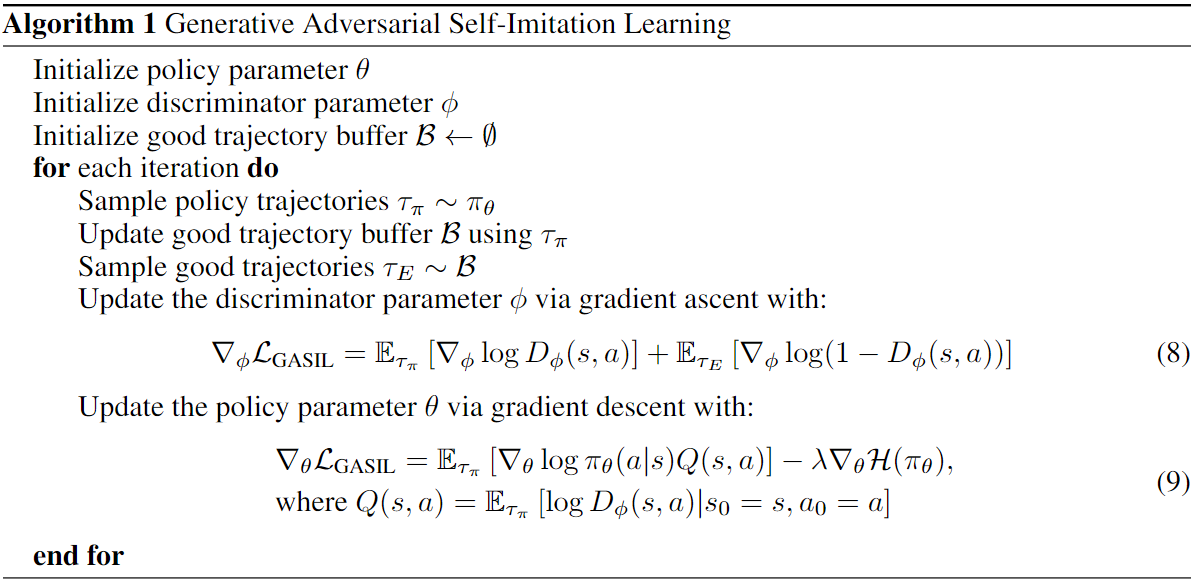
\includegraphics[width = \textwidth]{algorithm.png}
\end{figure}
where the good trajectories here are defined as historical top-K trajectories, and the gradient with respect to $\theta$ is actually to calculate the expectation's
gradient, which is discussed in the policy gradient section. Since the similarity between the policy's training and policy gradient, the $\log(D_\phi(s,a))$ here can be
regarded as a reward of an action $a$ given a state $s$. Therefore, GASIL can be easily combined with some policy gradient algorithms. So we can update the policy
parameter $\theta$ via gradient ascent with:
$$\nabla_\theta J_{PG}-\alpha\nabla_\theta L_{GASIL}=\mathbb{E}_{\pi_\theta}[\nabla_\theta\log(\pi_\theta(a|s)\hat A_t^\alpha)]$$
where $\hat A_t^\alpha$ is an advantage estimation using a modified reward function $r^\alpha(s,a)=r(s,a)-\alpha\log(D_\phi(s,a))$.
\section{Experiments}
The GASIL+PPO performs better than PPO, PPO+BC and PPO+SIL most of the time, and expecially performs well in the delayed environment:
\begin{figure}[H]
    \centering
    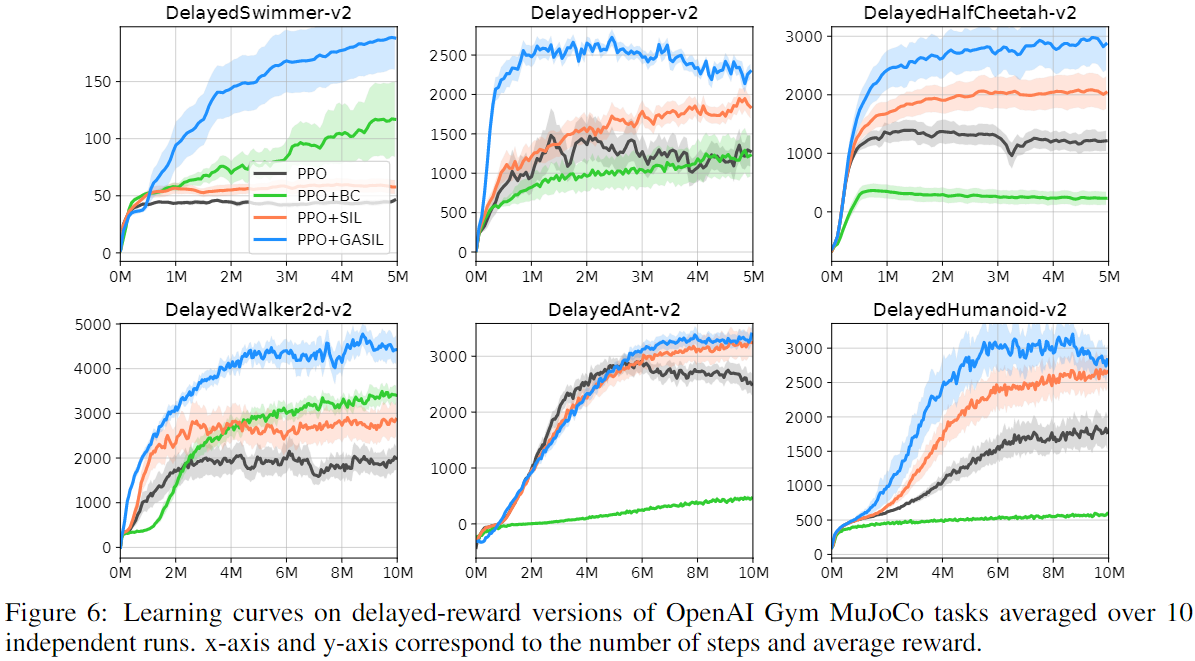
\includegraphics[width = \textwidth]{delay.png}
\end{figure}
since although the updating of accumulated reward is delayed, the updating of $\log(D_\phi(s,a))$ which can be also seen as a reward is immediate. Additionally, the
effect of hyperparameters is similar with GANs:
\begin{figure}[H]
    \centering
    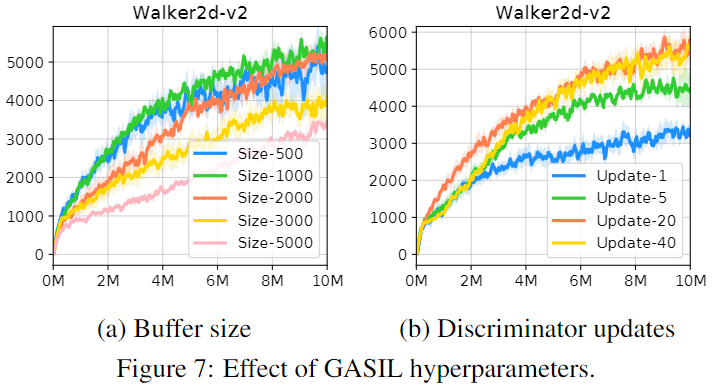
\includegraphics[width = 0.5\textwidth]{hyper.png}
\end{figure}
\section{Shortcomings And Future works}
\begin{enumerate}
    \item The current approach to training the discriminator is to simply discriminate top-K trajectories and generated trajectories, but the approch can be more
    theoretical.
    \item Exploit other policy instead of Gaussian policy to deal with the multi-modal trajectories problem.
    \item Introduce model-based methods such as MGAIL to make it more sample-efficient.
\end{enumerate}

%\clearpage
%\bibliography{E:/Papers/LiuLab}
%\bibliographystyle{apalike}
\end{document}
%%% Local Variables:
%%% mode: latex
%%% TeX-master: t
%%% End:
